\documentclass[a4paper,12pt,singlespacing]{article}
% Arquivo de configurações do modelo
\usepackage[T1]{fontenc}
\usepackage[utf8]{inputenc}
\usepackage[lmargin=2cm, rmargin=2cm, tmargin=2.5cm, bmargin=2.5cm]{geometry}
% \usepackage[brazil, brazilian]{babel}
\usepackage[style=abnt]{biblatex}
\usepackage{csquotes, graphicx, xcolor, comment, enumerate, multirow, multicol, titlesec, amsmath, amsthm, amsfonts, amssymb, dsfont, mathtools, blindtext, ragged2e, array, enumitem, tikz, bbding, pifont, wasysym, amssymb, hyperref, titling}
\newcommand{\cmark}{\ding{51}}
\newcommand{\xmark}{\ding{55}}

\tolerance=1
\emergencystretch=\maxdimen
\hyphenpenalty=10000
\hbadness=10000

\usepackage{helvet}
\renewcommand{\familydefault}{\sfdefault}

\usepackage{setspace}
\setlength{\JustifyingParindent}{1.25cm}
\setlength{\RaggedRightParindent}{0pt}
\setlength{\parskip}{6pt}

\usepackage{fancyhdr}
\pagestyle{fancy}
\fancyhf{}
\lhead{}
\rhead{}
\rfoot{\small\thepage}
\renewcommand{\headrulewidth}{0pt}

\titlespacing*{\section}{0pt}{6pt}{0pt}
\titlespacing*{\subsection}{0pt}{6pt}{0pt}
\titlespacing*{\subsubsection}{0pt}{6pt}{0pt}

\renewcommand{\thesection}{\arabic{section}.}
\renewcommand{\thesubsection}{\arabic{section}.\arabic{subsection}.}
\renewcommand{\thesubsubsection}{\arabic{section}.\arabic{subsection}.\arabic{subsubsection}.}

\titleformat{\section}{\normalsize\bfseries}{\makebox[1.25cm][l]{\thesection}}{0pt}{}
\titleformat{\subsection}{\normalsize\bfseries}{\makebox[1.25cm][l]{\thesubsection}}{0pt}{}
\titleformat{\subsubsection}{\normalsize\bfseries}{\makebox[1.25cm][l]{\thesubsubsection}}{0pt}{}

\usepackage{textcase}
\usepackage[font=small, labelsep=endash, textfont=bf, labelfont=bf, aboveskip=6pt, belowskip=-6pt, tablename=TABELA, figurename=FIGURA]{caption}
\usepackage[font=small, labelsep=endash, textfont=bf, labelfont=bf, aboveskip=6pt, belowskip=3pt, labelformat=simple]{subcaption}

\renewcommand{\thetable}{\arabic{table}}
\renewcommand{\thefigure}{\arabic{figure}}
\renewcommand{\thesubfigure}{\arabic{subfigure}}
\renewcommand{\thesubtable}{\arabic{subtable}}

\addbibresource{ref.bib}


% Utilizado para correções e comentários. Vá para 'util.tex' para saber mais.
\usepackage[normalem]{ulem}
\usepackage{color}
\usepackage[T1]{fontenc}

% Uso: \comando{texto}, onde 'comando' pode ser 'entra', 'sai', 'rever', 'todo', ou \comando[nota adicional]{texto}

\newcommand{\entra}[2][]{
   {\color{blue}#2}
   \ifx&#1&
      {}
    \else
      \footnote{{\color{blue}(entra):} #1}
    \fi
}

\newcommand{\sai}[2][]{
   {\color{black}\sout{#2}}
   \ifx&#1&
      {}
    \else
      \footnote{{\color{black}(sai):} #1}
    \fi
}

\newcommand{\rever}[2][]{
   {\color{magenta}#2}
   \ifx&#1&
      {}
    \else
      \footnote{{\color{magenta}(rever):} #1}
    \fi
}

\newcommand{\todo}[2][]{
   {\color{red}[ \textbf{TODO}: \textit{#2} ]}
   \ifx&#1&
      {}
    \else
      \footnote{{\color{red}(todo):} #1}
    \fi
}

\newcommand{\etal}{{\sl et~al.}}

\newcommand{\<}{\textrm{<}}
\renewcommand{\>}{\textrm{>}}


% Aqui devem ser inseridas as informações sobre o trabalho
    % Título:
    \title{PROJECT DESIGN III: PJD 301B}
    % Alunos e orientadores:
    \author{DESIGN DOCUMENTATION}
    % E-mails dos integrantes:
    \def\emails{e-mail do aluno 1, e-mail do aluno 2, e-mail do aluno 3, e-mail do Orientador, e-mail do Coorientador}

% Na pasta 'artigo' estão as respectivas seções que devem constar no trabalho. Lá deve ser inserido todo o conteúdo.

% Para referências, consulte 'ref.bib' e saiba mais. Na seção de Referencial Teórico, são exemplificadas as formas de se fazer uma citação.

\begin{document}
    {\centering
		\begin{figure}[!ht]
			\centering
			
\includegraphics[scale=0.15]{./tut_logo.png}
		\end{figure}

        \setlength{\parskip}{0pt}
		FACULTY OF INFORMATION \\ AND \\  COMMUNICATION TECHNOLOGY

        \setlength{\parskip}{18pt}
		NATIONAL DIPLOMA: COMPUTER SYSTEMS ENGINEERING

        \setlength{\parskip}{18pt}
        \textbf{ \thetitle }
        \setlength{\parskip}{12pt}

        \theauthor

        \setlength{\parskip}{6pt}
        % \footnotesize{\emails}

    }


    \clearpage  % Certification ended, now start a new page
    \tableofcontents
    \clearpage  % Certification ended, now start a new page


    \justifying

    % \section*{Resumo}

\noindent
% Resumo
Apresentar o texto do resumo em um único parágrafo (bloco único, sem recuo à esquerda). O resumo deve apresentar, de forma breve, o tema e sua importância, os objetivos, o marco teórico principal, a metodologia e os resultados alcançados. Logo, se apresenta no resumo uma visão clara do conteúdo e das conclusões do trabalho destacando os pontos relevantes. O resumo deve ser apresentado contendo entre 200 e 300 palavras. O texto do resumo e das palavras-chave são apresentados em fonte arial tamanho 12, com alinhamento do texto justificado e espaçamento de parágrafo em 6 pt antes e 6 pt depois. O espaçamento entre linhas é simples. Logo após o resumo são apresentadas as 3 (três) palavras-chave que representam o conteúdo do trabalho. Os termos “Resumo” e “Palavraschave” são apresentados em negrito e são alinhados à esquerda. Após o termo “Palavraschave” é inserido o sinal de dois pontos “:” para identificar o início das palavras selecionadas. As palavras são separadas entre si por ponto-e-vírgula “;” e após a última é inserido o ponto final “.”.

\noindent\textbf{Palavras-chave:}
% Palavras-chave
Palavra 1; Palavra 2; Palavra 3.


    \subsection{Introduction}

% \subsubsection{\textit{Purpose}}
The following document outline all design documentation of the smart livestock monitoring
System. This document is separated in section, you can jump to any specific section you want to learn more
about related to the livestock monitoring system. You are advice to read this document if you want to
learn more about the design principle and choices of the livestock monitoring system. The information on this document will
enable you to not only understand the system but will tell you how to trouble shoot the system if anything went
wrong and also extend the functionality of the system if you so choose to.

\subsubsection{\textit{Scope}}
The document will cover design consideration, Assumptions, goals and guideline. It will give you enough information
about Architectural strategies, System architectural and Functional flow of the livestock monitoring system.

\subsubsection{\textit{Audience}}
The design documentation is for anyone who want to learn more about the livestock monitoring system,
How it is design from ground up and how they can extend the system to solve other problem. This document it also
good for any engineers who want to replicate the system on their own.

% Apresentar o texto do objetivo. Em caso de utilização de lista, eis um exemplo:
% \begin{itemize}[noitemsep, topsep=0pt]
%     \item item 1;
%     \item item 2;
%     \item item 3.
% \end{itemize}


    \subsection{Systems overview}

The smart livestock monitoring system track livestock using ESP32 Micro controller. One ESP32 per
each livestock that contain a unique identify (UID) that will enable the system to count the total
livestock at a given time. A web sever connect to a database take the information sends sends by
the Micro controller and store it to a database.

The Micro controller is  being package to a case with a battery. The band that
cover the animal is a solar panel that charge the
battery so that it does not die quick. The case is that package the microcontroller is strong enough
to resist hard weather condition


    \section{Design considerations (1/2 page)}

This section describes many of the issues which need to be addressed or
resolved before attempting to devise a complete design solution.


    \clearpage  % Certification ended, now start a new page

    \section{Assumptions and dependencies (1/2 page)}

Describe any assumptions or dependencies regarding the software and hardware and their use. These may concern such issues as related software and hardware, end user characteristics etc
\subsection{Related software and hardware}
Describe the relative software and hardware.
\subsection{End-user characteristics}
Possible and/or probable changes in functionality
\subsection{General Constraints}

Describe any global limitations or constraints that have a significant impact on the design of the system's software (and describe the associated impact). Such constraints may be imposed by any of the following (the list is not exhaustive):

    • Hardware or software environment
    • End-user environment
    • Availability or volatility of resources
    • Other requirements described in the requirements specification


    \section{Goals and guidelines (1/2 page)}

Describe any goals, guidelines, principles, or priorities which dominate or embody the design of the system's software. Such goals might be:

    • The KISS principle ("Keep it simple stupid!")
    • Emphasis on speed versus memory use
    • Working, looking, or "feeling" like an existing product

For each such goal or guideline, unless it is implicitly obvious, describe the reason for its desirability. Feel free to state and describe each goal in its own sub-subsection if you wish.


    \clearpage  % Certification ended, now start a new page

    \subsection{Development Methods}

The development of the project is developed using two well known development methods in the
software industry, which is \textit{Agile development methodology} and \textit{DevOps deployment methodology}
Those methods was adapted after the first Software Development Life Cycle was applied.
The first step. Agile development methodology was used because it focus strongly on user experience
and input. This make the software high responsive to changes while developing the software and also
get the system up and factional quickly to meet the user needs. DevOps deployment methodology was to make
sure that I get the application up and running quick, using things such as continues deliverance, git and github.

\subsubsection{\textit{Planning}}

The first step on the development of the livestock monitoring system was to draft steps and
calculating labor cost and material costs, creating timetable with target goals and creating a
structure that can be followed when developing the system


\subsubsection{\textit{Creating}}

On this stage I focus more on packing the ESP32 to the case, connect the ESP to the WI-FI,
carefully soldering the system components on the veroboard, ensuring neat circuit is built and the are
no short circuit that may cause blowing of the components

\subsubsection{\textit{Developing}}

At this stage is where I switch to following Agile development methodology, since it is
a software problems. I developed a NodeJS sever using JavaScript and a framework called
Express.

\subsubsection{\textit{Deployment}}

I use git to deploy the application to the cloud. push the changes to git so that the system
can get the changes when made to the master branch. Tested the changes if the meet the user
needs that I define or proposed



    \subsection{Architectural Strategies}

The hardware is packaged on a black case of about 50cm to 20cm and 10cm hight. The case
for the hardware is light in weight and most of the livestock such as cattle and cow, sheep would not
feel the case weight. The decision I do not want to strain wight of the livestock that it end up
affect their growth

On the drawing board, I wanted a flexible solar pane to be used  as belt, that will
serve two purposes, Charge the battery inside the case and also hold the case in place
due to availability I only able to find a hard solar panel that can charge up to 6V.
This will affect the design, The final package, The case and all would look nice, but it will
be good enough to do a demonstration


\subsubsection{\textit{Tehchnologies used}}

The hardware, ESP32 Micro controller it is programmed using the C++ programming
language and the curl library was used to allow the ESP32 to communicate with
the server over the internet. C++ is the standard programming language when it
come to programming low level system, It can integrate very well with hardware.
Made sense to use C++ although is not the only language since we have
language such as C\# and Rust. C++ turned out to even have more advantage since
we also want to consume less power and it can be optimize to maximise the speed
of the CPU. Curl, is a open source library used in most C++ code base when need
to connect to the internet it is also light libra, it does not consume too much
power

The server, is developed with the JavaScript programming language using a
framework called Express. Running on a node server(the application). JavaScript
it has replaced PHP when you want to create a quick server. It has most security
feature and the is more resources online for libraries for absolute
anything you might want to do. The server is hosted on Linode, a cloud base
company that offer most cloud services. This is to make sure you can connect
to sever from anywhere around the world

Future plan for the application is to collect more data from the livestock such as temperature,
location and display the information in to the dashboard. Research on maximizing power efficient so that
the system can last longer on a single charge if the solar panel can not charge the battery in a
rainy weather.

The user interact with the system via a web browser. If they know how to user a web browser
They will know how to use the system. The input to the system is the signal sent from the case
to the server and the output will be the dashboard where we display the information about
the livestock


\subsubsection{\textit{Communication mechanisms used}}
\begin{figure}[htbp]
\centering
    \begin{subfigure}[b]{7cm}
        \centering
        % Primeira subfigura
        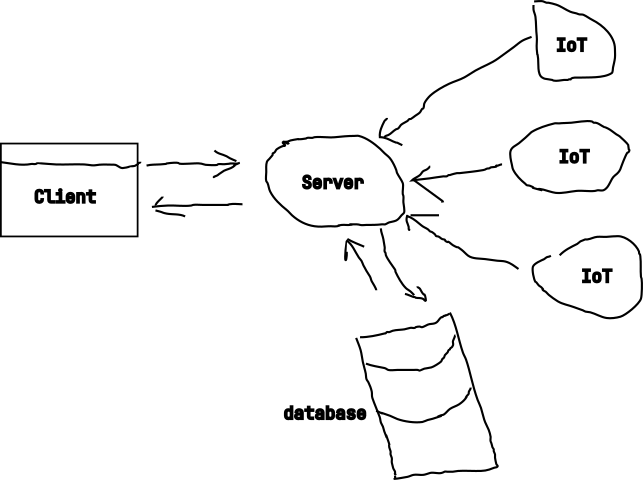
\includegraphics[width=7cm]{cc.png} % URI da subfigura
        \subcaption{
        % Legenda da subfigura
        data flow
        }
        \label{fig2:sub1}
    \end{subfigure}
\quad
    \begin{subfigure}[b]{7cm}
        \centering
        % Segunda subfigura
        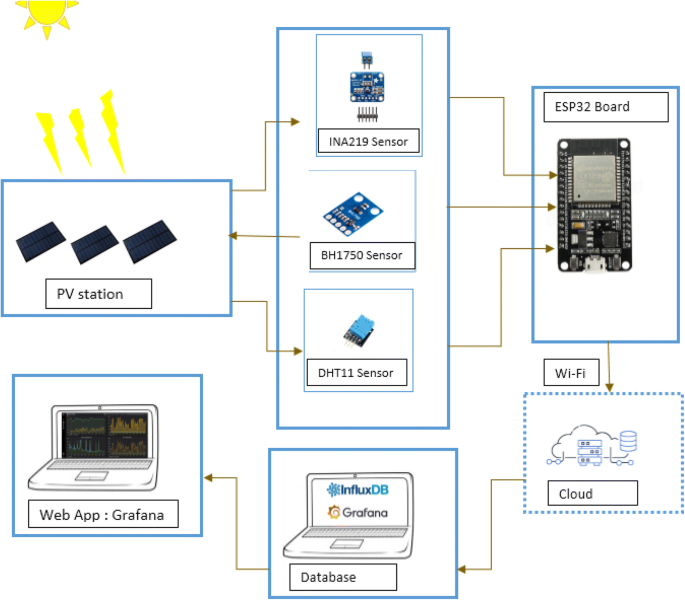
\includegraphics[width=7cm]{ccc.png} % URI da subfigura
        \subcaption{
        % Legenda da subfigura
        connection flow
        }
        \label{fig2:sub2}
    \end{subfigure}
\caption{
Communication diagram
}
\label{fig:fig2} % Tag para referência
\end{figure}

\subsection{Subsystem Architecture}

The system does not contain complicated componentes, everything is simple as it
archieve a specific things. This is by design, Thanks to the Unix philosophy. The
whole purpose of the system is to count livestock remotely


\subsubsection{\textit{ESP32(hardware)}}

For the system to be able to count livestock, E=each esp32 micro controller
get atatched to the livestock. The ESP32 the sends request to a remote server
with a uniquer UUID to identify the livestock. The request is being constantly send
to the server at an interval time rate

\subsubsection{\textit{Node Js (Server Application)}}

The Server application is connect to a Maria database and listening to HTTP request,
when a POST request is being made with UID, It gets save to the database with the time
stamp. The Server also expose a Web Socket to stream the total number of unique ID that are in the database.
When a client is connected to that socket, the total number its get send to the client

\subsubsection{\textit{Web Application (Client dashborad)}}
The Web applicaton connect to the server using web socket to listen to the datat bieng screaed from
the server which represent the number of unique ID from the databas



    \subsection{Functional Flow}

Provide a detailed description of the different system functions. For each
function provide an activity diagram, process flow table and a status flow
table.

Process Flow Table: In this table you list the processes in that function and a
description explaining the process

Status Flow Table: In this table you list the different statuses and add a
description to explain the status.
artictle/9-functional-flow.tex


    \subsection{Glossary}
Wow, My amazing list of definition, I hope you have like cathing up

artictle/11-glossary.tex


    \subsection{Bibliography}

 Wow, this is my amazing biblegraph
 artictle/12-bibliography.tex


\end{document}
